% vim: set textwidth=120:

% Example CV based on the 1.5-column-cv template. Main features:
% * uses the Roboto font family and IcoMoon icon set;
% * doesn't use colours, different font weights are used instead for styling;
% * because the CV fits on one page, header and footer is empty, since there isn't much useful info to put there;
% * includes a photo.
\documentclass[a4paper,10pt]{article}


% package imports
% ---------------

\usepackage[british]{babel} % for correct language and hyphenation and stuff
\usepackage{calc}           % for easier length calculations (infix notation)
\usepackage{enumitem}       % for configuring list environments
\usepackage{fancyhdr}       % for setting header and footer
\usepackage{fontspec}       % for fonts
\usepackage{geometry}       % for setting margins (\newgeometry)
\usepackage{graphicx}       % for pictures
\usepackage{microtype}      % for microtypography stuff
\usepackage{xcolor}         % for colours
\usepackage[colorlinks = true,
            linkcolor = blue,
            urlcolor  = blue,
            citecolor = blue,
            anchorcolor = blue]{hyperref}


% margin and column widths
% ------------------------

% margins
\newgeometry{left=15mm,right=15mm,top=15mm,bottom=15mm}

% width of the gap between left and right column
\newlength{\cvcolumngapwidth}
\setlength{\cvcolumngapwidth}{3.5mm}

% left column width
\newlength{\cvleftcolumnwidth}
\setlength{\cvleftcolumnwidth}{44.5mm}

% right column width
\newlength{\cvrightcolumnwidth}
\setlength{\cvrightcolumnwidth}{\textwidth-\cvleftcolumnwidth-\cvcolumngapwidth}

% set paragraph indentation to 0, because it screws up the whole layout otherwise
\setlength{\parindent}{0mm}


% style definitions
% -----------------
% style categories explanation:
% * \cvnameXXX is used for the name;
% * \cvsectionXXX is used for section names (left column, accompanied by a horizontal rule);
% * \cvtitleXXX is used for job/education titles (right column);
% * \cvdurationXXX is used for job/education durations (left column);
% * \cvheadingXXX is used for headings (left column);
% * \cvmainXXX (and \setmainfont) is used for main text;
% * \cvruleXXX is used for the horizontal rules denoting sections.

% font families
\defaultfontfeatures{Ligatures=TeX} % reportedly a good idea, see https://tex.stackexchange.com/a/37251

\newfontfamily{\cvnamefont}{Roboto Medium}
\newfontfamily{\cvsectionfont}{Roboto Medium}
\newfontfamily{\cvtitlefont}{Roboto Medium}
\newfontfamily{\cvdurationfont}{Roboto Light Italic}
\newfontfamily{\cvheadingfont}{Roboto Medium}
\setmainfont{Roboto Light}

% colours
\definecolor{cvnamecolor}{HTML}{00008e}
\definecolor{cvsectioncolor}{HTML}{00008e}
\definecolor{cvtitlecolor}{HTML}{000000}
\definecolor{cvdurationcolor}{HTML}{555555}
\definecolor{cvheadingcolor}{HTML}{000000}
\definecolor{cvmaincolor}{HTML}{000000}
\definecolor{cvrulecolor}{HTML}{000000}

\color{cvmaincolor}

% styles
\newcommand{\cvnamestyle}[1]{{\Large\cvnamefont\textcolor{cvnamecolor}{#1}}}
\newcommand{\cvsectionstyle}[1]{{\normalsize\cvsectionfont\textcolor{cvsectioncolor}{#1}}}
\newcommand{\cvtitlestyle}[1]{{\large\cvtitlefont\textcolor{cvtitlecolor}{#1}}}
\newcommand{\cvdurationstyle}[1]{{\small\cvdurationfont\textcolor{cvdurationcolor}{#1}}}
\newcommand{\cvheadingstyle}[1]{{\normalsize\cvheadingfont\textcolor{cvheadingcolor}{#1}}}


% inter-item spacing
% ------------------

% vertical space after personal info and standard CV items
\newlength{\cvafteritemskipamount}
\setlength{\cvafteritemskipamount}{5mm plus 1.25mm minus 1.25mm}

% vertical space after sections
\newlength{\cvaftersectionskipamount}
\setlength{\cvaftersectionskipamount}{2mm plus 0.5mm minus 0.5mm}

% extra vertical space to be used when a section starts with an item with a heading (e.g. in the skills section),
% so that the heading does not follow the section name too closely
\newlength{\cvbetweensectionandheadingextraskipamount}
\setlength{\cvbetweensectionandheadingextraskipamount}{1mm plus 0.25mm minus 0.25mm}


% intra-item spacing
% ------------------

% vertical space after name
\newlength{\cvafternameskipamount}
\setlength{\cvafternameskipamount}{3mm plus 0.75mm minus 0.75mm}

% vertical space after personal info lines
\newlength{\cvafterpersonalinfolineskipamount}
\setlength{\cvafterpersonalinfolineskipamount}{2mm plus 0.5mm minus 0.5mm}

% vertical space after titles
\newlength{\cvaftertitleskipamount}
\setlength{\cvaftertitleskipamount}{1mm plus 0.25mm minus 0.25mm}

% value to be used as parskip in right column of CV items and itemsep in lists (same for both, for consistency)
\newlength{\cvparskip}
\setlength{\cvparskip}{0.5mm plus 0.125mm minus 0.125mm}

% set global list configuration (use parskip as itemsep, and no separation otherwise)
\setlist{parsep=0mm,topsep=0mm,partopsep=0mm,itemsep=\cvparskip}


% CV commands
% -----------

% creates a "personal info" CV item with the given left and right column contents, with appropriate vertical space after
% @param #1 left column content (should be the CV photo)
% @param #2 right column content (should be the name and personal info)
\newcommand{\cvpersonalinfo}[2]{
    % left and right column
    \begin{minipage}[t]{\cvleftcolumnwidth}
        \vspace{0mm} % XXX hack to align to top, see https://tex.stackexchange.com/a/11632
        \raggedleft #1
    \end{minipage}% XXX necessary comment to avoid unwanted space
    \hspace{\cvcolumngapwidth}% XXX necessary comment to avoid unwanted space
    \begin{minipage}[t]{\cvrightcolumnwidth}
        \vspace{0mm} % XXX hack to align to top, see https://tex.stackexchange.com/a/11632
        #2
    \end{minipage}

    % space after
    \vspace{\cvafteritemskipamount}
}

% typesets a name, with appropriate vertical space after
% @param #1 name text
\newcommand{\cvname}[1]{
    % name
    \cvnamestyle{#1}

    % space after
    \vspace{\cvafternameskipamount}
}

% typesets a line of personal info beginning with an icon, with appropriate vertical space after
% @param #1 parameters for the \includegraphics command used to include the icon
% @param #2 icon filename
% @param #3 line text
\newcommand{\cvpersonalinfolinewithicon}[3]{
    % icon, vertically aligned with text (see https://tex.stackexchange.com/a/129463)
    \raisebox{.5\fontcharht\font`E-.5\height}{\includegraphics[#1]{#2}}
    % text
    #3

    % space after
    \vspace{\cvafterpersonalinfolineskipamount}
}

% creates a "section" CV item with the given left column content, a horizontal rule in the right column, and with
% appropriate vertical space after
% @param #1 left column content (should be the section name)
\newcommand{\cvsection}[1]{
    % left and right column
    \begin{minipage}[t]{\cvleftcolumnwidth}
        \raggedleft\cvsectionstyle{#1}
    \end{minipage}% XXX necessary comment to avoid unwanted space
    \hspace{\cvcolumngapwidth}% XXX necessary comment to avoid unwanted space
    \begin{minipage}[t]{\cvrightcolumnwidth}
        \textcolor{cvrulecolor}{\rule{\cvrightcolumnwidth}{0.3mm}}
    \end{minipage}

    % space after
    \vspace{\cvaftersectionskipamount}
}

% creates a standard, multi-purpose CV item with the given left and right column contents, parskip set to cvparskip
% in the right column, and with appropriate vertical space after
% @param #1 left column content
% @param #2 right column content
\newcommand{\cvitem}[2]{
    % left and right column
    \begin{minipage}[t]{\cvleftcolumnwidth}
        \raggedleft #1
    \end{minipage}% XXX necessary comment to avoid unwanted space
    \hspace{\cvcolumngapwidth}% XXX necessary comment to avoid unwanted space
    \begin{minipage}[t]{\cvrightcolumnwidth}
        \setlength{\parskip}{\cvparskip} #2
    \end{minipage}

    % space after
    \vspace{\cvafteritemskipamount}
}

% typesets a title, with appropriate vertical space after
% @param #1 title text
\newcommand{\cvtitle}[1]{
    % title
    \cvtitlestyle{#1}

    % space after
    \vspace{\cvaftertitleskipamount}
    % XXX need to subtract cvparskip here, because it is automatically inserted after the title "paragraph"
    \vspace{-\cvparskip}
}


% header and footer
% -----------------

% set empty header and footer
\pagestyle{empty}



% preamble end/document start
% ===========================

\begin{document}


% personal info
% -------------

\cvpersonalinfo{
    % photo
    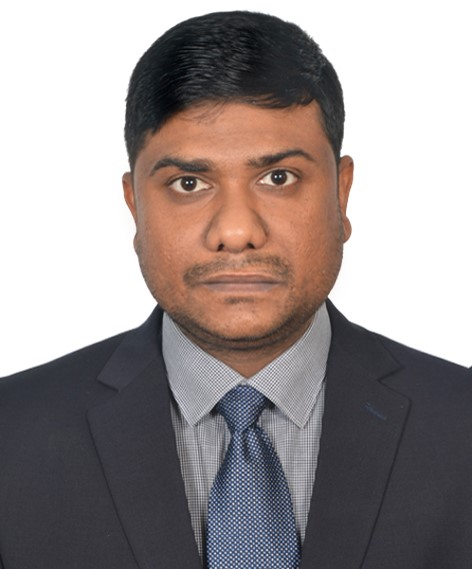
\includegraphics[height=36mm]{Passport Photo-resized.jpg}
}{
    % name
    \cvname{Md. Farukuzzaman Faruk}
    % address
   {
      PhD Candidate in Computer Science,
         School of Computing \& Informatics,\\
         University of Louisiana at Lafayette. \\
     }
    % phone number
    \cvpersonalinfolinewithicon{height=4mm}{067-phone.pdf}{
        +1 337-557-3009    }
    % email address
    \cvpersonalinfolinewithicon{height=4mm}{070-envelop.pdf}{
    md-farukuzzaman.faruk1@louisiana.edu, faarukuzzaman@gmail.com
    }

    % LinkedIn account
    \cvpersonalinfolinewithicon{height=4mm}{1011424-internet.png}{
        \href{https://scholar.google.com/citations?user=NAE84dMAAAAJ&hl=en}{Google Scholar}
    }
    \cvpersonalinfolinewithicon{height=4mm}{1011424-internet.png}{
        \href{https://www.ruet.ac.bd/farukuzzaman}{https://www.ruet.ac.bd/farukuzzaman}
    }

    % date of birth
    % \textbf{Date of Birth:} 1 June 1992 %1015, 146000
}

\cvsection{OBJECTIVES}
\cvitem{
    \cvdurationstyle{}
}
{
To build a career as a computer science researcher, advancing knowledge through impactful research, addressing modern challenges, and exploring cutting-edge technologies, with a commitment to continuous learning, adaptation, and meaningful contributions to global technological progress.}


% work experience
% ---------------

\cvsection{WORK EXPERIENCE}

% Fake Company 2
\cvitem{
    \cvdurationstyle{}
}
{\textbf{Total Teaching Experience: 6+ Years }}

\cvitem{
    \cvdurationstyle{Aug 2025 -- Current}
}{
    \cvtitle{Graduate Teaching Assistant $\cdot$ Full Time}

    School of Computing \& Informatics,\\
    University of Louisiana at Lafayette, LA, USA.
}


\cvitem{
    \cvdurationstyle{Jul 2022 -- Jul 2025}
}{
    \cvtitle{Assistant Professor $\cdot$ Full Time}

    Department of Computer Science \& Engineering,\\
    RUET, Rajshahi-6204, Bangladesh
}

% Fake Company 1
\cvitem{
    \cvdurationstyle{Nov 2019 -- Jul 2022}
}{
    \cvtitle{Lecturer $\cdot$ Full Time}

    Department of Computer Science \& Engineering,\\
    RUET, Rajshahi-6204, Bangladesh
}

\cvitem{
    \cvdurationstyle{Feb 2019 -- Oct 2019}
}{
    \cvtitle{Lecturer $\cdot$ Full Time}

    Department of Computer Science \& Engineering,\\
    Varendra University, Rajshahi, Bangladesh
}

% education
% ---------

\cvsection{EDUCATION}

% % pd.d
% \cvitem{
%     \cvdurationstyle{2023 -- Current}
% }{
%     \cvtitle{ Pursuing Phd in Computer Science \& Engineering}
    
%     Department of Computer Science, Stony Brook University, NY, USA
% }

% PhD
\cvitem{
    \cvdurationstyle{2025 -- Ongoing}
}{
    \cvtitle{PhD in  Computer Science}
    
    School of Computing \& Informatics,\\
    University of Louisiana at Lafayette, LA, USA.

}

% master's
\cvitem{
    \cvdurationstyle{2019 -- 2021}
}{
    \cvtitle{Master of Science in Computer Science \& Engineering}
    CGPA: \textbf{3.92} (out of 4.00)\\
    Department of Computer Science \& Engineering,RUET, Rajshahi-6204, Bangladesh
    \vspace{2mm}\\
    \textbf{Thesis Topic:} Deep Convolutional Neural Network-based Medical Images Analysis.\\
     \textbf{Supervisor:} Prof. Dr. Md. Rabiul Islam, Dept. of CSE, RUET
}

% bachelor's
\cvitem{
    \cvdurationstyle{2014 -- 2018}
}{
    \cvtitle{Bachelor of Science in Computer Science \& Engineering}
    CGPA: \textbf{3.90} (out of 4.00), Position: \textbf{Third} (Out of 106 Students)\\
    Department of Computer Science \& Engineering,
    RUET, Rajshahi-6204, Bangladesh
    \vspace{2mm}\\
     \textbf{Thesis Topic:} Prediction of DNA Methylation Status Using Support Vector Machine. \\
     \textbf{Supervisor:} Prof. Dr. A H M Sarowar Sattar, Dept. of CSE, RUET
}


% skills
% ------

\cvsection{SKILLS \& INTERESTS}

\vspace{\cvbetweensectionandheadingextraskipamount}

% fake skills
\cvitem{
    \cvheadingstyle{Research Interests}
}{
   Machine Learning, Deep Learning, Natural Language Processing, Medical Image Processing, Biomedical Signal Processing
}

% languages
\cvitem{
    \cvheadingstyle{Languages}
}{
    English -- Full professional proficiency(\textbf{IELTS Score: 6.5)}, Bengali -- Full professional proficiency
}

\cvitem{
    \cvheadingstyle{Interpersonal Skills}
}{
    Presentation, Documentation, Public Speaking, Time and Event Management
}

\cvitem{
    \cvheadingstyle{Programming Languages}
}{
    C, C++, Python,  PHP, JAVA, JavaScript
}
\cvitem{
    \cvheadingstyle{Platforms/Frameworks}
}{
    Jupyter Notebook, Google Colab, Kaggle, Pycharrm, TensorFlow
}
\cvsection{PUBLICATIONS}
% \vspace{\cvbetweensectionandheadingextraskipamount}

% \cvitem{
%     \cvdurationstyle{}
% }
% %{\textbf{Journal: 1, Conference Papers: 38}}

\cvitem{
    \cvheadingstyle{Selected Publications}
} {
   Md. Farukuzzaman Faruk, Abu Sayeed, “K-mer Based DNA Methylation Status Prediction Using Support Vector Machine”, In 3rd International Conference on Electrical, Computer, and Telecommunication Engineering (ICECTE), 26-28 December 2019, Rajshahi, Bangladesh. (\textbf{Received IEEE Bangladesh Section Best Paper Award})
\vspace{2mm}\\
Md Farukuzzaman Faruk, Md Rabiul Islam, and Emrana Kabir Hashi. "Screening pathological abnormalities in gastrointestinal images using deep ensemble transfer learning." In 2022 25th International Conference on Computer and Information Technology (ICCIT), pp. 230-235. IEEE, 2022.
\vspace{2mm}\\
  Farukuzzaman Faruk. "Vggcovidnet: A deep convolutional neural network to predict covid-19 cases from x-ray images." In 2021 International Conference on Automation, Control and Mechatronics for Industry 4.0 (ACMI), pp. 1-6. IEEE, 2021.
\vspace{2mm}\\
Farukuzzaman  Faruk. "Rgu-net: Residual guided u-net architecture for automated segmentation of covid-19 anomalies using ct images." In 2021 International Conference on Automation, Control and Mechatronics for Industry 4.0 (ACMI), pp. 1-6. IEEE, 2021.
\vspace{2mm}\\
Md Farukuzzaman  Faruk. "Residualcovid-net: An interpretable deep network to screen covid-19 utilizing chest ct images." In 2021 3rd International Conference on Electrical & Electronic Engineering (ICEEE), pp. 69-72. IEEE, 2021
\vspace{2mm}\\
 Mrinmoy Mondal, Md Farukuzzaman Faruk, Nasif Raihan, and Protiva Ahammed. "Deep transfer learning based multi-class brain tumors classification using mri images." In 2021 3rd International Conference on Electrical & Electronic Engineering (ICEEE), pp. 73-76. IEEE, 2021.
 \vspace{2mm}\\
 Protiva Ahammed, Md Farukuzzaman Faruk, Nasif Raihan, and Mrinmoy Mondal. "Inception V3 Based Transfer Learning Model for the Prognosis of Acute Lymphoblastic Leukemia from Microscopic Images." In 2022 4th International Conference on Electrical, Computer & Telecommunication Engineering (ICECTE), pp. 1-4. IEEE, 2022.
\vspace{2mm}\\
 Anirban Barai, Md. Farukuzzaman Faruk, Shakil Mahmud Shuvo, Azmain Yakin Srizon, S. M. Mahedy Hasan and Abu Sayeed. "A Late Fusion Deep CNN Model for the Classification of Brain Tumors from Multi-Parametric MRI Images." In 2023 International Conference on Next-Generation Computing, IoT and Machine Learning (NCIM), pp. 1-6. IEEE, 2023.
\vspace{2mm}\\
 Shakil Mahmud Shuvo, Md Farukuzzaman Faruk, Azmain Yakin Srizon, Tahsen Islam Sajon, SM Mahedy Hasan, Anirban Barai, A. F. M. Minhazur Rahman, and Md Al Mamun. "Multi-class Brain Tumor Classification with DenseNet-Based Deep Learning Features and Ensemble of Machine Learning Approaches." In International Conference on Big Data, IoT and Machine Learning, pp. 559-573. Singapore: Springer Nature Singapore, 2023.
\vspace{2mm}\\
Md Sabbir  Hossain, Md Farukuzzaman Faruk, Azmain Yakin Srizon, SM Mahedy Hasan, Md Shariful Chowdhury, Md Rakib Hossain, Md Nazmul Islam, and Md Faruk Hossain. "A Customized 3D CNN Integrated with Convolutional Block Attention Module for Precise Diagnosis of COVID-19 and Pneumonia from CT Scan Images." In 2023 26th International Conference on Computer and Information Technology (ICCIT), pp. 1-6. IEEE, 2023.
\vspace{2mm}\\
Barsha Roy, Md Farukuzzaman Faruk, Md Nazmul Islam, Azmain Yakin Srizon, SM Mahedy Hasan, Md Al Mamun, Md Rakib Hossain, and Md Faruk Hossain. "A Cutting-Edge Ensemble of Vision Transformer and ResNet101v2 Based Transfer Learning for the Precise Classification of Leukemia Sub-types from Peripheral Blood Smear Images." In 2024 6th International Conference on Electrical Engineering and Information & Communication Technology (ICEEICT), pp. 49-54. IEEE, 2024.

}
\cvitem{
    \cvheadingstyle{Selected Publications}
} {

Farjana Islam, Md Farukuzzaman Faruk, SM Mahedy Hasan, Farzana Akter, Azmain Yakin Srizon, Md Rakib Hossain, Md Al Mamun, Md Nazmul Islam, and Md Faruk Hossain. "An Investigation of Hyperparameters Optimization and Feature Reduction Techniques: Predicting Airline Passenger Satisfaction Using Machine Learning Models." In 2023 26th International Conference on Computer and Information Technology (ICCIT), pp. 1-6. IEEE, 2023.
\vspace{2mm}\\
 Ishmam Khan, Azmain Yakin Srizon, Md Farukuzzaman Faruk, Md Al Mamun, SM Mahedy Hasan, Md Nazmul Islam, Md Rakib Hossain, and Md Faruk Hossain. "Leveraging the Robust Capability of Modified Multi-Layer Gated Recurrent Units for Fake News Detection." In 2024 6th International Conference on Electrical Engineering and Information & Communication Technology (ICEEICT), pp. 986-991. IEEE, 2024.
\vspace{2mm}\\
Sirajam Samira, Md Farukuzzaman Faruk, Md Nazmul Islam, SM Mahedy Hasan, Md Al Mamun, Azmain Yakin Srizon, and Md Rakib Hossain. "Enhancing Gastrointestinal Diagnosis: CBAM-Integrated CNN for High-Precision Multi-Class Anatomical Landmark Identification." In 2024 Second International Conference on Emerging Trends in Information Technology and Engineering (ICETITE), pp. 1-6. IEEE, 2024.
\vspace{2mm}\\
Abu Sayeed, Nasif Osman Khansur, Azmain Yakin Srizon, Md Farukuzzaman Faruk, Salem A Alyami, AKM Azad, Mohammad Ali Moni,"An effective screening of COVID‐19 pneumonia by employing chest X‐ray segmentation and attention‐based ensembled classification", Journal of IET Image Processing, 2024. Access DOI: 10.1049/ipr2.13106 
\vspace{2mm}\\
     Md Nazmul Islam, Md Al Mamun, Md Farukuzzaman Faruk, Azmain Yakin Srizon, SM Mahedy Hasan, and Barsha Roy. "Spatial Attention-guided Deep Learning for Accurate Kidney Disease Classification in CT Scans." In 2023 26th International Conference on Computer and Information Technology (ICCIT), pp. 1-6. IEEE, 2023.
    \vspace{2mm}\\
    Md Ahsan Habib Raj, Md Al Mamun, and Md Farukuzzaman Faruk. "CNN based diabetic retinopathy status prediction using fundus images." In 2020 IEEE region 10 symposium (TENSYMP), pp. 190-193. IEEE, 2020
    }
%\newpage
\cvsection{TRAINING \& WORKSHOPS}

\vspace{\cvbetweensectionandheadingextraskipamount}

% fake skills
\cvitem{
    \cvheadingstyle{Training}
}
{
Foundation Training on Teaching-Learning (19-22 September 2020, Organized by RUET, Rajshahi, Bangladesh)

}
\cvitem{
    \cvheadingstyle{Workshops}
}{
Workshop on BQNF and BAC Accreditation (19-28 June 2021, Organized by RUET, Rajshahi, Bangladesh)
}
\cvsection{HONORS \& MEMBERSHIPS}

\vspace{\cvbetweensectionandheadingextraskipamount}

% fake skills

\cvitem{
    \cvheadingstyle{Awards}
}{
    \begin{itemize}
    \item{IEEE Bangladesh Section Best Paper Award in 3rd International Conference on Electrical, Computer, and Telecommunication Engineering, 2019, Organized by Faculty of ECE, RUET, Rajshahi-6204, Bangladesh}
    \item{University Merit Scholarship (Duration: Total four year of undergraduate study)}
    \end{itemize}
}

\cvitem{
    \cvheadingstyle{Professional Consultancies}
}{
    \begin{itemize}
    \item Consultant for Software Development and Maintenance of Rajshahi WASA(Fiscal year 2021-22,
2022-23 and 2023-24).
    \end{itemize}
}

\cvitem{
    \cvheadingstyle{Organizing Committee Member}
}{
 \begin{itemize}
        \item Member, Organizing Committee, IEEE PEEIACON Conference-2024.
        \item Member, Technical and Organizing Committee, RUET CSE Fest 2K22.
\end{itemize}
}

% additional info
% ---------------
\cvsection{SUPERVISION \& MANAGEMENT}
\cvitem{
    \cvheadingstyle{Supervision}
}{
     I have supervised more than 15 undergraduate student’s thesis work.
}
\cvitem{
    \cvheadingstyle{Management}
}{
\begin{itemize}
    \item Deputy Director of Students’ Welfare (Finance), RUET (Sep, 2023 to Aug 2024)\\
    \item Assistant Provost, Shahid Lt. Selim Hall, RUET (Feb 2021 to Sep 2023)\\
\end{itemize}
    
}
%\newpage

\cvsection{FUNDED PROJECTS}
% \cvitem{
%     \cvheadingstyle{[1]}
% }{
%     \textbf{Project Name: Deep Convolution Neural Network Based Medical Images Segmentation.}\\
%     \textbf{Resposibily: Project Director}\\
%     Duration: July 2020 to June 2021 (Completed)\\
%     Funding: 150,000 BDT, Funded By: University Grants Commission of Bangladesh(UGC) and Office of the Director of Research \& Extension, RUET.
% }
\cvitem{
    \cvheadingstyle{[1]}
}{
    \textbf{Project Name: Diagnosis of COVID-19 Cases Using Deep Network from Chest Images.}\\
    \textbf{Resposibily: Project Director}\\
    Duration: July 2021 to June 2022 (Completed)\\
    Funding: 150,000 BDT, Funded By: University Grants Commission of Bangladesh(UGC) and Office of the Director of Research \& Extension, RUET.
}
\cvitem{
    \cvheadingstyle{[2]}
}{
    \textbf{Project Name: Fast and Automatic Approach
for the Detection of Gastrointestinal Diseases
Using Deep Network.}\\
    \textbf{Resposibily: Project Director}\\
    Duration: July 2022 to June 2023 (Completed)\\
    Funding: 150,000 BDT, Funded By:  University Grants Commission of Bangladesh(UGC) and Office of the Director of Research \& Extension, RUET.
}
\cvitem{
    \cvheadingstyle{[3]}
}{
    \textbf{Project Name: Synergistic Ensemble:
Integrating Vision Transformer and ResNet-101
for the Precise Classification of Leukemia
Subtypes.}\\
    \textbf{Resposibily: Project Director}\\
    Duration: July 2023 to June 2024 (Completed)\\
    Funding: 150,000 BDT, Funded By: Funded By:  University Grants Commission of Bangladesh(UGC) and Office of the Director of Research \& Extension, RUET.
}
\cvitem{
    \cvheadingstyle{[4]}
}{
    \textbf{Project Name: Exploiting the Robust Features of Adapted Multi-Layer Gated Recurrent Units for
Comprehensive Fake News Identification.}\\
    \textbf{Resposibily: Project Director}\\
    Duration: Ongoing\\
    Funding: 150,000 BDT, Funded By: Funded By:  University Grants Commission of Bangladesh(UGC) and Office of the Director of Research \& Extension, RUET.}
\cvsection{RELEVANT COURSEWORKS}
\cvitem{
    \cvheadingstyle{Undergraduate Courses}
}{
    Computer Programming (C),
    Data Structures,
    Object Oriented Programming (OOP),
    Discrete Mathematics,
    Computer Algorithms,
    Database System,
    Computer Network,
    Software Engineering,
    Microprocessors \& Assembly Language,
    Operating System,
    Artificial Intelligent,
    Digital Image Processing,
    Digital Signal Processing,
    Computer Graphics,
    Neural Networks \& Fuzzy Systems,
    Network Security, Data Mining
}
\cvitem{
    \cvheadingstyle{Postgraduate Courses}
}{
    Advanced Artificial Intelligence,
    Advanced Digital Image Processing,
    Biometrics,
    Pattern Recognition,
    Software Project Management,
    Computer Arithmetic Analysis\
}


\end{document}